%----------------------------------------------------------------------------------------
%	PACKAGES AND OTHER DOCUMENT CONFIGURATIONS
%----------------------------------------------------------------------------------------


\documentclass[a4paper]{article}
\usepackage[a4paper, total={6in, 8in}]{geometry}
\usepackage[utf8]{inputenc} % Required for inputting international characters
\usepackage[T1]{fontenc} % Output font encoding for international characters
\usepackage[pdftex]{graphicx}     
\usepackage{mathpazo} % Palatino font
\usepackage[section]{placeins}
\usepackage[labelsep=quad,indention=10pt]{subfig}
\usepackage{url}
\usepackage{physics}
\newcommand\tab[1][1cm]{\hspace*{#1}}
\newcommand\sbullet[1][.5]{\mathbin{\vcenter{\hbox{\scalebox{#1}{$\bullet$}}}}}
\usepackage{amsmath}
\usepackage{color, colortbl}
\usepackage{tabularx,ragged2e,booktabs,caption}
\usepackage[table,x11names]{xcolor}
\usepackage[first=0,last=9]{lcg}
\newcommand{\ra}{\rand0.\arabic{rand}}
\captionsetup*[subfigure]{position=bottom}
\usepackage{tikz}
\usetikzlibrary{tikzmark}
\usepackage{float}
\usepackage{dblfloatfix}
\usepackage[english]{babel}

\addto\captionsenglish{% Replace "english" with the language you use
  \renewcommand{\contentsname}%
    {Sadržaj}%
}

\captionsetup[table]{name=Tablica}
\addto\captionsenglish{\renewcommand{\figurename}{Slika.}}

\begin{document}

%----------------------------------------------------------------------------------------
%	TITLE PAGE
%----------------------------------------------------------------------------------------

\begin{titlepage} % Suppresses displaying the page number on the title page and the subsequent page counts as page 1
	\newcommand{\HRule}{\rule{\linewidth}{0.5mm}} % Defines a new command for horizontal lines, change thickness here
	
	\center % Centre everything on the page
	
	%------------------------------------------------
	%	Headings
	%------------------------------------------------
	
	\textsc{\LARGE Fakultet elektrotehnike i računarstva}\\[1.5cm] % Main heading such as the name of your university/college
	
	\textsc{\Large Bioinformatika}\\[0.5cm] % Major heading such as course name
	
	
	
	%------------------------------------------------
	%	Title
	%------------------------------------------------
	
	\HRule\\[0.4cm]
	
	{\huge\bfseries Određivanje poravnanja parova sljedova korištenjem HMM}\\[0.4cm] % Title of your document
	
	\HRule\\[1.5cm]
	
	%------------------------------------------------
	%	Author(s)
	%------------------------------------------------
	
	\begin{minipage}{0.4\textwidth}
		\begin{flushleft}
			\large
			\textit{Autori}\\
			 {Tomislav Božurić}\\
			 {Martin Pisačić}\\
			 {Krešimir Topolovec} % Your name
		\end{flushleft}
	\end{minipage}
	~
	\begin{minipage}{0.4\textwidth}
		\begin{flushright}
			\large
			\textit{Mentor}\\
			 doc. dr. sc. {Mirjana Domazet-Lošo} % Supervisor's name
		\end{flushright}
	\end{minipage}
	
	% If you don't want a supervisor, uncomment the two lines below and comment the code above
	%{\large\textit{Author}}\\
	%John \textsc{Smith} % Your name
	
	%------------------------------------------------
	%	Date
	%------------------------------------------------
	
	\vfill\vfill\vfill % Position the date 3/4 down the remaining page
	
	{\large Siječanj, 2019} % Date, change the \today to a set date if you want to be precise
	
	%------------------------------------------------
	%	Logo
	%------------------------------------------------
	
	\vfill\vfill
	
\includegraphics[width=0.4\textwidth]{fer_logo.jpg}\\[1cm] % Include a department/university logo - this will require the graphicx package
	 
	%----------------------------------------------------------------------------------------
	
	\vfill % Push the date up 1/4 of the remaining page
	
\end{titlepage}
\tableofcontents
\newpage
\section{Opis algoritma i vizualizacija}
U ovome radu korišten je modificirani Viterbijev algoritam pomoću kojeg korištenjem dinamičkog programiranja možemo pronaći najvjerojatniju sekvencu skrivenih stanja koja ujedno predstavlja optimalno poravnanje dvaju nizova. \\

\subsection{Primjena Viterbijevog algoritma na Pair-HMM}

Da bismo klasičan Viterbijev algoritam tranformirali u Pair-HMM, moramo napraviti nekoliko izmjena. Prvo moramo odrediti vjerojatnosti za emitiranje simbola iz pojedinih stanja prikazanih na dijagramu \ref{fig:hmm}. Npr. stanje $M (match)$ ima vjerojatnosnu distribuciju $p_{ab}$ za emitaranje para simbola $ab$. Stanja $X$ i $Y$ imaju vjerojatnost emitiranja $q_a$ simbola $a$ i praznine u drugi niz. Dakle, ako iz stanja $X$ emitiramo simbol $x_{i}$ s vjerojatnošču $q_{x_{i}}$, u suprotni niz se ubacuje praznina. Nužno je potrebno definirati vjerojatnosti prijelaza između stanja tako da je suma vjerojatnosti odlaska iz pojedinog stanja jednaka 1. Vjerojatnost prijelaza iz stanja M u stanje X i Y opisujemo oznakom $\delta$, a vjerojatnost u ostanka u stanju X ili Y sa $\epsilon$.
Takva definicija ne definira kompletni model koji omogućava vjerojatnosnu distribuciju po svim mogućim sekvecama. Za kompletiranje modela dodajemo početno i krajnje stanje $Pocetak$ i $Kraj$. Također, definiramo vjerojatnost $\tau$ koja je jednaka za sve prijelaze iz stanja $M$, $X$ i $Y$ u stanje $End$, te za stanje $Begin$ u stanja $M$.
Iz razloga što ovakav tip modela generira dva poravnata niza nazivamo ga engl. pair HMM kako bi ga razlikovali od standardnih HMM koji generiraju jedan niz. 

\noindent
\\
Generiranje nizova počinje iz stanja $Begin$ i cirkulira između dva koraka i stanja ${M,X,Y}$ sve dok proces ne dostigne stanje $End$. Navedena dva koraka su:
\begin{itemize}
    \item odaberi novo stanje prema distribuciji vjerojatnosti prijelaza iz trenutnog stanja
    \item odaberi par simbola koji se dodaje u poravnanje prema definiranoj distribuciji vjerojatnosti emitiranja simobla
\end{itemize}

\noindent
Bitno je uočiti da različita poravnanja mogu imati različite duljine zbog ovisnosti o distribuciji vjerojatnosti. Kako je vjerojatnost prijelaza iz stanja $M$, $X$ ili $Y$ u stanje $End$ jednaka $\tau$, očekivana duljina nizova jednaka je ${1}/{\tau}$.

\begin{figure}[H]
  \includegraphics[width=\textwidth]{HMM.png}
  \caption{Model HMM-a korištenog za poravnanje parova sekvenci}
  \label{fig:hmm}
\end{figure}

\noindent
\subsection{Algoritam: Viterbijev algoritam za HMM \cite{hmm_algorithms}}
Viterbijev algoritam dati će najvjerojatniji put kroz skrivena stanja u pair HMM. 
\newline\newline
Inicijalizacija: \\
\tab \tab $v^M(0,0) = 1$\\
\tab \tab $v^{\sbullet[.75]}(i,0) = v^{\sbullet[.75]}(0,j) = 0$\\
Korak:\\
\tab za svaki $i=1,...,n$, $j=1,...,m$ \\
\begin{equation}
     v^M(i,j) = p_{x_iy_i} \max
    \begin{cases}
      (1 - 2\delta - \tau)v^M(i-1,j-1)\\
      (1-\epsilon-\tau)v^X(i-1,j-1)\\
      (1-\epsilon - \tau)v^Y(i-1,j-1)\\          
    \end{cases}
\end{equation}
\begin{equation}
     v^X(i,j) = q_{x_i}\max
    \begin{cases}
      \delta v^M(i-1,j)\\
      \epsilon v^X(i-1,j)\\
    \end{cases}   
\end{equation}
\begin{equation}
     v^Y(i,j) = q_{y_j}\max
    \begin{cases}
      \delta v^M(i,j-1)\\
      \epsilon v^Y(i,j-1)\\
    \end{cases}   
\end{equation}
Uvjet zaustavljanja:
$v^E = \max(v^M(n,m), v^X(n,m), v^Y(n,m))$ \\

\noindent
Iz navedenih koraka jasno je da se radi o formi algoritma sličnoj kao kod poravnanja slijedova dinamičkim programiranjem. Možemo reči da Viterbijev algoritam spada u skupinu algoritama koji koriste dinamičko programiranje.

\noindent
Zbog činjenice da su vjerojatnosti brojevi u intervalu $[0,1]$, gore navedeni algoritam nije upotrebiv za implementaciju na računalu zbog velikog broja množenja brojeva bliskih nuli, pa se u praksi koristi logaritamska inačica tog algoritma koja je navedena u nastavku.  

\noindent
\\
\subsection{Algoritam: optimalno poravnanje logaritamskih kvota \cite{hmm_algorithms}}  

Inicijalizacija: 
\tab \tab $V^M(0,0) = - 2 log(\eta), V^X(0,0) = V^Y(0,0) = -\infty$\\
\tab \tab $V^{\sbullet[.75]}(i,-1) = V^{\sbullet[.75]}(-1,j) = -\infty$\\
Korak:\\
\tab za svaki $i=0,...,n$, $j=0,...,m$ osim (0,0):\\
\begin{equation}
     V^M(i,j) = s(x_i,y_j) + \max
    \begin{cases}
      V^M(i-1,j-1)\\
      V^X(i-1,j-1)\\
      V^Y(i-1,j-1)\\          
    \end{cases}
\end{equation}
\begin{equation}
     V^X(i,j) = \max
    \begin{cases}
      V^M(i-1,j) - d\\
      V^X(i-1,j) - e\\
    \end{cases}   
\end{equation}
\begin{equation}
     V^Y(i,j) = \max
    \begin{cases}
      V^M(i,j-1) -d\\
      V^Y(i,j-1) - e\\         
    \end{cases}
\end{equation}
Uvjet zaustavljanja:
$V = \max(V^M(n,m), V^X(n,m) + c , V^Y(n,m) + c )$ \\
Pri čemu su:\\
	\tab$s(a,b) = \log\frac{p_{ab}}{q_a q_b} + \log\frac{1 - 2\delta - \tau }{(1-\eta)^2}$\\
    \tab$d = -\log\frac{\delta(1-\epsilon - \tau)}{(1-\eta)(1-2\delta - \tau)}$\\
    \tab$e = -\log\frac{\epsilon}{1-\eta}$\\
	\tab$c = \log( 1 - 2\delta - \tau) - \log(1-\epsilon - \tau)$
	
	
	
\begin{center}
\centering
\captionof{table}{Vizualizacija početnog stanja matrice $V_M$} \label{tab:title} 
  \begin{tabular}{ | >{\columncolor[gray]{0.8}}c | c | c | c | c | c | c |}
    \hline
     \rowcolor{lightgray} indeks & -1 & 0 & 1 & 2 & ... & m\\ \hline
     -1 & $-\infty$ & $-\infty$ & $-\infty$  & $-\infty$  & $-\infty$  & $-\infty$   \\ \hline
      0 & $-\infty$ & $-2log\eta$ & &  &  &\\ \hline
      1 & $-\infty$  & & & & &\\  \hline
      2 & $-\infty$  & & & & &\\ \hline
      ... & $-\infty$ & & & & &\\ \hline
      n & $-\infty$ & & & & &\\ \hline
      \end{tabular}
\end{center}

U tablici iznad možemo vidjet početno stanje matrice u kojoj pamtimo logaritamske kvote za stanje podudaranja. Iz modificiranog Viterbijevog algoritma koji koristiti logaritamske kvote iterativno korištenjem dinamičkog programiranja punimo tablicu i upisujemo novo izračunate vrijednosti. Analogno radimo za tablice ispod, te kada dođemo do kraja iste te tablice koristimo za rekonstrukciju optimalnog poravnanja. Želimo li izračunati primjerice za vrijednosti $i=1, j=0$ izraz za $V_M$ bi izgledao ovako: \\ 
\begin{equation}
     V^M(1,0) = s(x_1,y_0) + \max
    \begin{cases}
      V^M(0,-1) = -\infty\\
      V^X(0,-1) = -\infty\\
      V^Y(0,-1) = -\infty\\          
    \end{cases}
\end{equation}
Analogno popunjavamo preostali dio tablice. Ovdje možemo primjetiti kako za računanje vrijednosti u koraku $i,j$ nam trebaju podatci iz koraka $i-1, j-1$, tako da je potrebno pararelno popunjavati sve tri prikazane matrice.

\begin{center}
\centering
\captionof{table}{Vizualizacija početnog stanja matrice $V_X$} \label{tab:title} 
  \begin{tabular}{ | >{\columncolor[gray]{0.8}}c | c | c | c | c | c | c |}
    \hline
     \rowcolor{lightgray} indeks & -1 & 0 & 1 & 2 & ... & m\\ \hline
     -1 & $-\infty$ & $-\infty$ & $-\infty$  & $-\infty$  & $-\infty$  & $-\infty$   \\ \hline
      0 & $-\infty$ & $-\infty$ & &  &  &\\ \hline
      1 & $-\infty$  & & & & &\\  \hline
      2 & $-\infty$  & & & & &\\ \hline
      ... & $-\infty$ & & & & &\\ \hline
      n & $-\infty$ & & & & &\\ \hline
            
\hline
  \end{tabular}
\end{center}


\begin{center}
\centering
\captionof{table}{Vizualizacija početnog stanja matrice $V_Y$} \label{tab:title} 
  \begin{tabular}{ | >{\columncolor[gray]{0.8}}c | c | c | c | c | c | c |}
    \hline
     \rowcolor{lightgray} indeks & -1 & 0 & 1 & 2 & ... & m\\ \hline
     -1 & $-\infty$ & $-\infty$ & $-\infty$  & $-\infty$  & $-\infty$  & $-\infty$   \\ \hline
      0 & $-\infty$ & $-\infty$ & &  &  &\\ \hline
      1 & $-\infty$  & & & & &\\  \hline
      2 & $-\infty$  & & & & &\\ \hline
      ... & $-\infty$ & & & & &\\ \hline
      n & $-\infty$ & & & & &\\ \hline
            
\hline
  \end{tabular}
\end{center}

Kada smo završili s forward dijelom algoritma, odnosno kada su nam sve strukture podatka popunjene spremni za pronalazak optimalnog poravnanja dvije sekvence. Kako nam je uvjet "zaustavljanja" $V = \max(V^M(n,m), V^X(n,m) + c , V^Y(n,m) + c )$, tražimo maksimum između navednih stanja. Zatim   generiramo poravnanje  te u povratku prema početku ponavljamo postupak tražeći maksimum između $V_M, V_X, V_Y$.Na idućem primjeru je ilustriran primjer pronalaska optimalnog poravnanja gdje se na poziciji $(n,m)$ vrijednost računa kako je prethodno spomenuto. \\

\begin{center}
\centering
\captionof{table}{Vizualizacija pronalaska optimalnog poravnanja} \label{tab:title} 
  \begin{tabular}{ | >{\columncolor[gray]{0.8}}c | c | c | c |c  | c | c | c |}
    \hline
      0 & 1 & 2 & 3 & ...& ... & m-1  & m\\ \hline
      0 & $V^{\sbullet[.75]}(0,0)$ \tikzmark{d}   & &  &   &  & &   \\ \hline
      1 &  &$V^{\sbullet[.75]}(1,1)$ \tikzmark{c}  &  &   &  &  & \\ \hline
      2 &  & &  &  &  &   &\\ \hline
      3 &  & &  &   &     & &  \\ \hline
      ... &  & &  &   & ...  & ... &    \\ \hline
      n-1 &  & &  &   & ... & $V^{\sbullet[.75]}(n-1,m-1)$ \tikzmark{b}&   \\ \hline
      n &  & &  &   &  &  & $V^{\sbullet[.75]}(n,m)$ \tikzmark{a}\\ \hline
            
   
            
\hline
  \end{tabular}
  
  \begin{tikzpicture}[overlay, remember picture, yshift=.40\baselineskip, shorten >=.5pt, shorten <=.5pt]
     \draw [->] ({pic cs:a}) [bend right] to ({pic cs:b});
      \draw [->] ({pic cs:c}) [bend right] to ({pic cs:d});
  \end{tikzpicture}
\end{center}

\subsection{Memorijski optimalniji algoritam optimalnih poravnanja logaritamskih kvota}
U prošlome poglavlju prikazali smo algoritam poravnanja logaritamskih kvota koji se često koristi u praksi jer vrijednosti iz iteracije u iteraciju ne iščezavaju kao što je to slučaj kod klasične vjerojatnosne izvedbe. Pogledamo li ponovno jednadžbe algoritma:\\\\
Korak:\\
\tab za svaki $i=0,...,n$, $j=0,...,m$ osim (0,0):\\
\begin{equation*}
     V^M(i,j) = s(x_i,y_j) + \max
    \begin{cases}
      V^M(i-1,j-1)\\
      V^X(i-1,j-1)\\
      V^Y(i-1,j-1)\\          
    \end{cases}
\end{equation*}
\begin{equation*}
     V^X(i,j) = \max
    \begin{cases}
      V^M(i-1,j) - d\\
      V^X(i-1,j) - e\\
    \end{cases}   
\end{equation*}
\begin{equation*}
     V^Y(i,j) = \max
    \begin{cases}
      V^M(i,j-1) -d\\
      V^Y(i,j-1) - e\\         
    \end{cases}
\end{equation*}

intuitivno je kako se za samo izvršavanje algoritma svi međurezultati mogu pohranjivati u 2D polja, iz kojih se u narednim koracima uzimaju prethodno izračunate vrijednosti. Prednost ovog pristupa svakako je njegova jednostavnost, no mana je što za veće instance sekvenci koje se poravnavaju memorija sve više raste, pri čemu računalo više nije niti u stanju pohraniti sve strukture u svoju radnu memoriju. No ovaj problem može se elegantno riješiti ako pogledamo jednadžbe koje ponavljamo iz koraka u korak. Pogledamo li malo bolje jednadžbe, vidimo da u nekome koraku $i$ i $j$ vrijednosti za taj korak računamo samo u ovisnost o vrijednostima iz prethodnoga koraka ili o vrijednostima iz trenutnoga koraka ali iz ranijih iteracija. Pošto prilikom programske implementacije vrijednosti $i$ i $j$ vrtimo kao dvije ugniježđene petlje, tako ćemo za svaku vrijednost $i$ proći kroz sve vrijednosti $j$ što se u našim indeksima uvijek odnosi na dvije vrijednosti iz ranije iteracije (označenih sa $i - 1$) te iz vrijednost trenutne iteracije (označenih sa $j - 1$).\\
Modificirana verzija algoritma radi na sljedeći način:

\begin{enumerate}
  \item Kreiraj 3 polja $M'$, $X'$, $Y'$ ukupne veličine $M$ 
  \item Inicijaliziraj vrijednosti polja na početne vrijednosti algoritma
  \item za svaki $i = 0,...,N$\\
        \tab kreiraj pomoćna polja $M_p'$, $X_p'$, $Y_p'$\\
        \tab za svaki $j = 0,...,M$\\
           \tab \tab ažuriraj:\\
            \tab \tab  $M_p'[j] = s(x_i,y_j)$ + $max(M'[j - 1], X'[j - 1], Y'[j - 1])$\\
            \tab \tab $X_p'[j] = max(M'[j - 1] - d, X'[j - 1] - e)$\\
            \tab \tab $Y_p'[j] = max(M_p'[j - 1] - d, Y_p'[j - 1] - e)$\\
        \tab kraj petlje\\
        \tab zamijeni: \\
        \tab \tab $M' \leftarrow M_p'$\\
        \tab \tab $X' \leftarrow X_p'$\\
        \tab \tab $Y' \leftarrow Y_p'$\\
        kraj petlje
 
\end{enumerate}



\subsection{Procjena parametara}
Parametre skrivenog Markovljevog modela procjenili smo statističkom metodom  maksimalne izglednosti parametara (\textit{Maximum Likelihood Estimation}) s zaglađivanjem nad bazom prikupljenih parova sekvenci ebole, hepatitisa, HIV-a, virusa bjesnoće i  tripomizina. Nakon procjena vjerojatnosti prijelaza iz stanja u stanje, kako naš skriveni Markovljev model koristi tri različite vjerojatnosti ($\delta, \tau , \epsilon$), prijelaze iz jednog stanja u neko drugo stanje smo odredili uprosječivanjem odgovarajućih prijelaza.\\
\begin{center}
$e(\alpha, \beta) = \frac{E(\alpha, \beta) + smoothing}{\sum_{\alpha, \beta} E(\alpha, \beta)  + 2\cdot smoothing}$
\end{center}

Gornju formulu koristimo za procjenu vjerojatnosti generiranja poravnatog para, odnosno za generiranje matrice vjerojatnosti emitiranja parova simbola. Primjerice za procjenu vjerojatnosti emitiranja para simbola (A,T) ili (C,G) analogno za sve ostale parove. Funkcija $E(\alpha, \beta)$ predstavlja broj pojavljivanja para ($\alpha, \beta$) u poravnatim sekevencama iz baze podataka za učenje. Sumu u nazivniku možemo lakše iterpretirati i kao duljinu poravnatih sekvenci. Parametar $smoothing$ je uveden kako bi i parovima koji se nisu pojavili u bazi podataka za učenje dodjelili određenu vjerojatnost, odnosno kako bi naš model postao robustniji, kako bi mu povećali efikasnu moć generalizacije i smanjili pretreniranost na podatke koje je već "vidio". 


\begin{center}
$t(X, Y) = \frac{T(X, Y) + smoothing}{\sum_{X, Y} T(X, Y)  + 2\cdot smoothing}$
\end{center}


Gornju formulu koristimo za procjenu vjerojatnosti priejlaza između stanja skrivenog Markovljevog modela. Kako smo već ustanovili da naš model koristi tri vjerojatnosti ($\delta, \tau, \epsilon$) nakon dobivene tranzicijske matrice korištenjem gornje formule za sve prijelaze između stanja koji imaju definiranu istu vjerojatnost računamo srednju vrijednost. U navednoj formuli $T(X,Y)$ označava broj prijelaza između stanja X u Y. Primjerice T(M,X) bi predstavljao koliko puta smo imali prijelaz između stanja M u X u bazi poravnatih sekvenci. Analogno suma u nazivniku predstavlja ukupan broj svih prijelaza u bazi poravnatih sekvenci. Analogno smo koristili $smoothing$ parametar kako bi model bolje generalizirao.


\section{Testiranje, analiza točnosti, vremena izvođenja i utroška memorije}
Vremenska i memorijska složenost modificiranog Viterbijevog algoritma jest $\mathcal{O}(NM)$. U svrhu analize točnosti algoritma korištena je usporedba  poravnanja s alatom MAFFT (\url{https://mafft.cbrc.jp/alignment/software/}).\\

\subsection{Testiranje performansi algoritma}
Za primjer testiranja performansi programa izvučeno je nekoliko parova sekvenci nad kojima smo izvršili dani algoritam te mjerili vrijeme izvođenja i memorijsku potrošnju. Primjeri su odabrani tako da predstavljaju sekvence različitih duljina kako bi vidjeli kako duljina sekvenci koje se poravnavaju utječe na same performanse algoritma. Kako je i predviđeno, što su sekvence koje se poravnavaju duže, tako je i trajanje izvođenja algoritma dulje, a memorijski utrošak veći.\\\\
Specifikacije računala na kojemu se algoritam izvršava su:
\begin{itemize}
  \item OS: Ubuntu 18.04.1 LTS 64 bit
  \item CPU: Intel® Core™ i7-7500U CPU @ 2.70GHz
  \item RAM: 12 GB DDR4, 2133 MHz
  \item Disk: Samsung 850 EVO SSD, brzina pisanja do 520 MB/s, brzina slijednog čitanja do 540 MB/s
\end{itemize}
Rezultati izvođenja algoritma dani su u tablici ispod:

\begin{table}[H]
\centering
\begin{tabular}{|c||p{3.9cm}|c|p{4.25cm}|c|p{1.cm}|p{1.5cm}|}
\hline
\# & \textit{\textbf{Sekvenca 1}} & \textit{\textbf{Duljina}} & \textit{\textbf{Sekvenca 2}} & \textit{\textbf{Duljina}} & \textit{\textbf{Vrijeme izvođenja}} & \textit{\textbf{Max utrošak memorije}} \\ \hline
1 & AF086833.2 Ebola virus - Mayinga, Zaire, 1976, complete genome & 18959 & JF828358.1 Lloviu virus strain MS-Liver-86/2003, complete genome & 18927 & 4,9 min / 297 s & 5 GiB \\ \hline
2 & HIV: Ref.A1 .RW .92 .92RW008 .AB253421 & 9643 & HIV:Ref.A1 .UG .92 .92UG037 .AB253429 & 9690 & 79 s / 76594 ms & 1,3 GiB \\ \hline
3 & AF384372.1 Hepatitis B virus isolate G376-A6, complete genome & 3125 & NC\_004102.1 Hepatitis C virus genotype 1, complete genome & 9646 & 25016 ms & 431,4 MiB \\ \hline
4 & FJ424484.1 Rabies virus red fox/08RS-1981/Udine/2008 nucleoprotein (N) gene, partial cds & 1350 & MG996466.1 Rabies lyssavirus isolate VIEV\_RV\_Dog\_69\_461\_2016 nucleoprotein gene, complete cds & 1353 & 1585 ms & 26,2 MiB \\ \hline
5 & embl:BF056441 BF056441; 7k05a04.x1 NCI\_CGAP\_GC6 Homo sapiens cDNA clone IMAGE:3443238 3' similar to SW:TPM4\_HUMAN P07226 TROPOMYOSIN, FIBROBLAST NON-MUSCLE TYPE ;, mRNA sequence. & 675 & embl:BE848719 BE848719; uw40c07.y1 Soares\_thymus\_2NbMT Mus musculus cDNA clone IMAGE:3419148 5' similar to SW:TPM4\_HUMAN P07226 TROPOMYOSIN, FIBROBLAST NON-MUSCLE TYPE ;, mRNA sequence. & 699 & 474 ms & 6.8 MiB \\ \hline
\end{tabular}
\caption{Trajanje izvođenja i memorijski utrošak izvođenja algoritma}
\label{table:trajanje}   
\end{table}

Koristeći memorijski optimiziranu verziju algoritma koja umjesto 2D polja čuva vrijednosti samo za prethodni i trenutni korak u vidu 1D polja, postigli smo puno manju iskoristivost memorije, a koja se najbolje vidim na većim instancama (pr. virus ebole). Ovim pristupom vrijeme izvođenja se nije promijenilo i vremenska složenost je ostala ista, no memorijska složenost se smanjila. Rezultati su prikazani u tablici ispod:

\begin{table}[H]
\centering
\begin{tabular}{|c||p{4cm}|p{4.25cm}|p{2cm}|p{2cm}|}
\hline
\# & \textit{\textbf{Sekvenca 1}} & \textit{\textbf{Sekvenca 2}} & \textit{\textbf{Vrijeme izvođenja}} & \textit{\textbf{Max utrošak memorije}} \\ \hline
1 & AF086833.2 Ebola virus - Mayinga, Zaire, 1976, complete genome & JF828358.1 Lloviu virus strain MS-Liver-86/2003, complete genome & 4,95 min / 297 s & 1,0 GiB \\ \hline
2 & HIV: Ref.A1 .RW .92 .92RW008 .AB253421 & HIV:Ref.A1 .UG .92 .92UG037 .AB253429 & 79 s / 76594 ms & 267,8 MiB \\ \hline
3 & AF384372.1 Hepatitis B virus isolate G376-A6, complete genome & NC\_004102.1 Hepatitis C virus genotype 1, complete genome & 25196 ms & 86,6 MiB \\ \hline
4 & FJ424484.1 Rabies virus red fox/08RS-1981/Udine/2008 nucleoprotein (N) gene, partial cds & MG996466.1 Rabies lyssavirus isolate VIEV\_RV\_Dog\_69\_461\_2016 nucleoprotein gene, complete cds & 1579 ms & 5,4 MiB \\ \hline
5 & embl:BF056441 BF056441; 7k05a04.x1 NCI\_CGAP\_GC6 Homo sapiens cDNA clone IMAGE:3443238 3' similar to SW:TPM4\_HUMAN P07226 TROPOMYOSIN, FIBROBLAST NON-MUSCLE TYPE ;, mRNA sequence. & embl:BE848719 BE848719; uw40c07.y1 Soares\_thymus\_2NbMT Mus musculus cDNA clone IMAGE:3419148 5' similar to SW:TPM4\_HUMAN P07226 TROPOMYOSIN, FIBROBLAST NON-MUSCLE TYPE ;, mRNA sequence. & 414 ms & 1,5 MiB \\ \hline
\end{tabular}
\caption{Trajanje izvođenja i memorijski utrošak izvođenja memorijski optimizirane verzije algoritma}
\label{table:economicSchools}   
\end{table}

Ono što možemo primjetiti je kako se memorija u svakoj instanci umanjila za otprilike 5 puta što je znatno osjetnije na većim instancama.

\subsection{Grafovi utroška memorije za navedene slučajeve}
U ovome podpoglavlju dajemo uvid u potrošnju memorije za svaki od gore navedenih slučajeva testiranja programa na parovima sekvenci. Ovdje možemo vidjeti koji djelovi algoritma troše najviše memorije, te što to znači za samu efikasnost i upotrebu algoritma. Grafove utroška prikazati ćemo na primjeru instance \textit{1} iz navedenih tablica.\\\\
U klasičnoj verziji algoritma za sva tri moguća stanja: \textit{M}, \textit{X}, \textit{Y} pratimo sve viđene vjerojatnosti u matricama dimenzija \textit{N} x \textit{M}, a memorijsku potrošnju možemo vidjeti na slici ispod:
\begin{figure}[H]
\centering
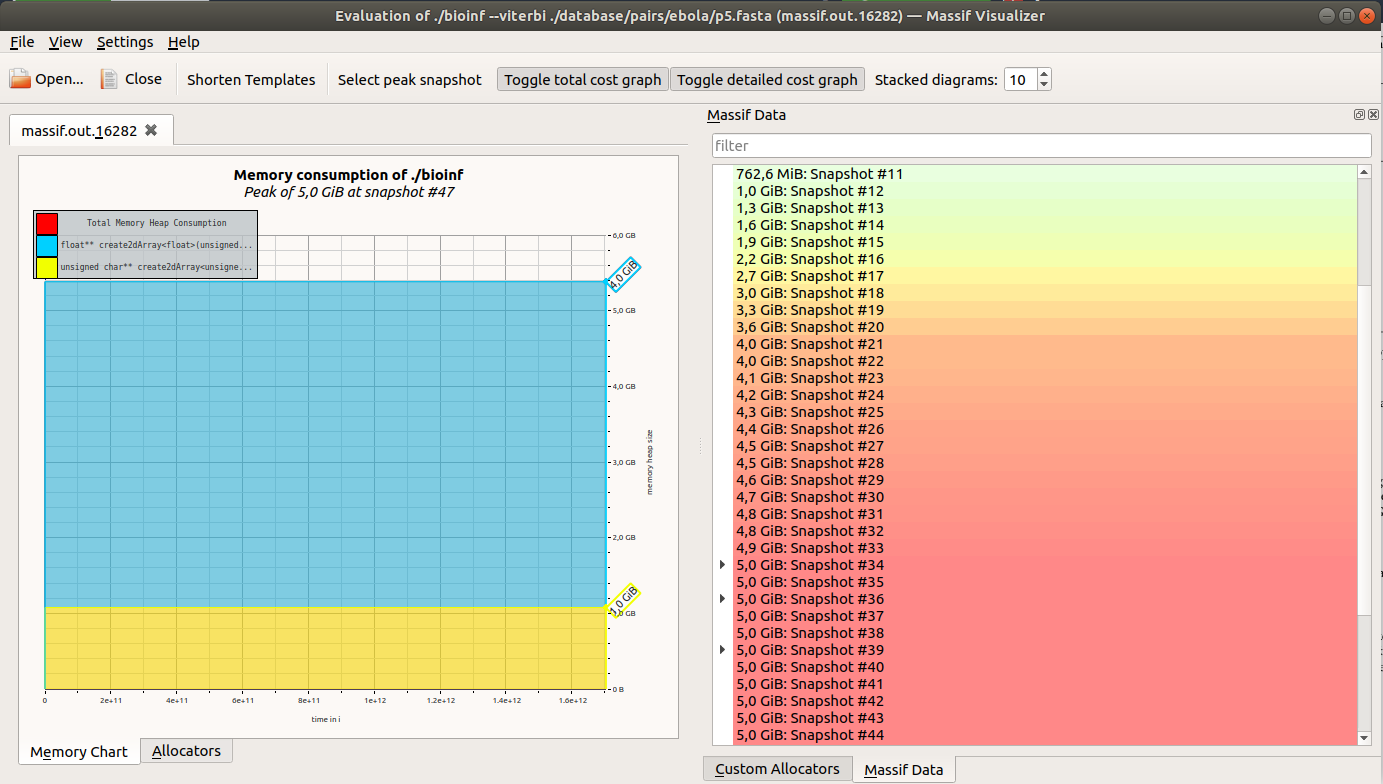
\includegraphics[width=\linewidth]{memory-consumption-classic.png}
\caption{Memorijska potrošnja klasičnog algoritma}
\end{figure}

Graf utroška memorije za optimizirani algoritam dan je na slici ispod:
\begin{figure}[H]
\centering
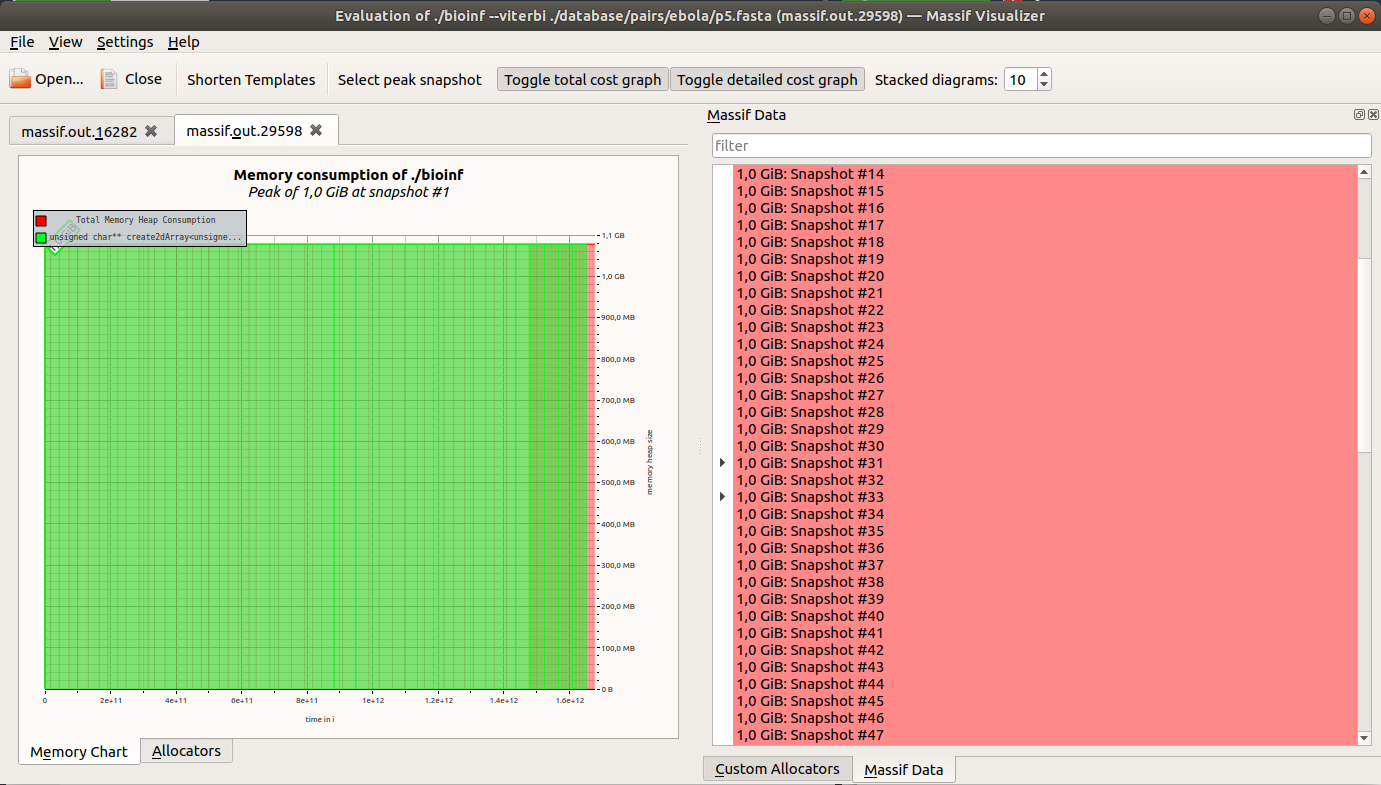
\includegraphics[width=\linewidth]{memory-consumption-optimized.png}
\caption{Memorijska potrošnja optimiziranog algoritma}
\end{figure}

Ono što također možemo primjetiti je i koje strukture zauzimaju najviše memorije, što je prikazano na slikama ispod:
\begin{figure}[H]
\centering
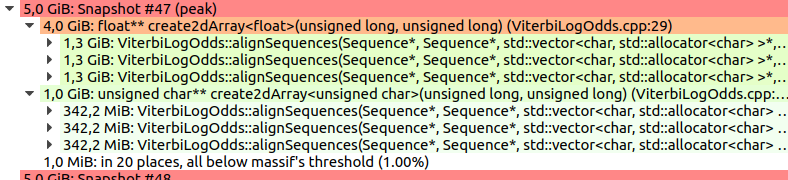
\includegraphics[width=\linewidth]{variables-classic.png}
\caption{Strukture podataka za klasični algoritam}
\end{figure}

Graf utroška memorije za optimizirani algoritam dan je na slici ispod:
\begin{figure}[H]
\centering
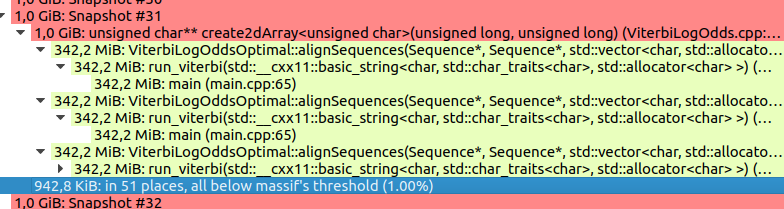
\includegraphics[width=\linewidth]{variables-optimal.png}
\caption{Strukture podataka za optimizirani algoritam}
\end{figure}

Kao što je i očekivano, 2D polja (matrice) zauzimaju više memorije no što to čine klasična polja.

\subsection{Analiza točnosti}

Za provjeru kvalitete rješenja računali smo \textit{score} na temelju supstitucijske tablice \textbf{Blosum62} i pri tome smo definirali kaznu za otvaranje praznine $-5$, i kaznu za produživanje praznine kao $-1$. Rezultate smo usporedili s alatom \textit{MAFFT} koji je očekivano dao bolje rezultate jer je naš model vjerojatnosne distribucije učio na ograničenoj bazi podataka pa sam procjena parametara ovisi o toj bazi poravnatih sekvenci. U nastavku su dane usporedbe za nekoliko sekvenci.
\begin{table}[H]
\centering
\begin{tabular}{|p{0.5\linewidth}|c| c|}
\hline
\multicolumn{1}{|c|}{\textit{\textbf{Sekvenca}}} & \multicolumn{1}{c|}{\textit{\textbf{Pairwise HMM score }}} & \multicolumn{1}{c|}{\textit{\textbf{MAFFT score}}}                                      \tabularnewline \hline
HIV:Ref.A1.RW.92.92RW008.AB253421, Ref.A1.UG.92.92UG037.AB253429 & $10296$ & $49486$  \\ \hline
AF086833.2 Ebola virus - Mayinga, Zaire, 1976, complete genome, JF828358.1 Lloviu virus strain MS-Liver-86/2003, complete genome & $13473$ & $46349$ \\ \hline
FJ424484.1 Rabies virus red fox, MG996466.1 Rabies lyssavirus  & 1268 & 7439 \\ \hline
Tropomyiosin : Homo sapiens cDNA, Soares Thymus Mus musculus cDNA & 545 & 1761 \\ \hline
Hepatitis B virus isolate G376-A6, complete genome, Hepatitis C virus genotype 1, complete genome & $-6504$  & $2691$\\ \hline
\end{tabular}
\caption{Usporedba rezultata poravnanja modela učenog na bazi više virusa poravnatoj s alatom \textit{MAFFT}}
\label{table:virusi}   
\end{table}
Nakon procjenjenih parametara na temelju baze poravnatih sekvenci ebole, hepatitisa, HIV-a, virusa bjesnoće i  tropomizina pokušali smo bazu podataka izgraditi koristeći alat \textit{ClustalW} nad parovima sekvenci HIV-a. Zatim smo iste te parove poravnali alatom \textit{MAFFT} i dobili smo približno jednake rezultate za poravnate sekvence  našeg modela i izlaza \textit{MAFFT}-a za različite sekvence.\\
\begin{table}[H]
\centering
\begin{tabular}{|p{0.5\linewidth}|c| c|}
\hline
\multicolumn{1}{|c|}{\textit{\textbf{Sekvenca}}} & \multicolumn{1}{c|}{\textit{\textbf{Pairwise HMM score }}} & \multicolumn{1}{c|}{\textit{\textbf{MAFFT score}}}                                      \tabularnewline \hline
HIV:Ref.A1.RW.92.92RW008.AB253421, Ref.A1.UG.92.92UG037.AB253429 & $46609$ & $49486$  \\ \hline
HIV:Ref.A1.RW.92.92RW008.AB253421, Ref.A2.CD.97.97CDKTB48.AF286238 & $36264$ & $42534$  \\ \hline
Tropomyiosin : Homo sapiens cDNA, Soares Thymus Mus musculus cDNA & 855 & 1761 \\ \hline
Hepatitis B virus isolate G376-A6, complete genome, Hepatitis C virus genotype 1, complete genome  &-3273 & 2691 \\ \hline
Nasumične sekvenca duljine 101 i 105 znakova  & 102 & 139 \\\hline
Nasumične sekvenca duljine 5097 i 5053 znakova  & 4300 & 8751 \\\hline

\end{tabular}
\caption{Usporedba rezultata poravnanja modela učenog na bazi HIV-a poravnatoj s \textit{ClustalW}-om }
\label{table:bazaHiv}   
\end{table}
Isproban je i model skrivenog Markovljevog modela učen na temelju baze poravatih sekvenci s alatom \textit{ClustalW} na virusima ebole i HIV-a, on je dao bolje rezultate kod poravnanja od prvog modela za viruse na kojima smo testirali (HIV, hepatitis i tropomizin), no bio je lošiji od modela učenog samo na bazi HIV-a s identičnim alatom.
\newpage
\section{Zaključak}
Završetkom projekta možemo reći da je bio vrlo izazovan i zanimljiv za rješavanje. Susreli smo se s proučavanjem znanstvenih članaka i njihovom implementacijom, iz prve ruke vidjeli kako memorijska i vremenska složenost utječu na izvršavanje programa te optimizacijom samih algoritama. Projekt je naposlijetku davao zadovoljavajuće rezultate poravnanja parova, iako mu je potrebno nešto više vremena nego klasičnim alatima (\textit{ClustalW, T-Coffe, ...}). Daljna poboljšanja bi mogla ići u smjeru pokušaja daljnje optimizacije utroška memorije i vremena, odnosno na dodatnu analizu samog koda i traženja točaka koje bi mogle pridonjeti ubrzanju rada algoritma. Dodatno, mogli bismo model učiti nad većom bazom parova poravnatih sekvenci kako bi bolje procijenili parametre  i napravili model robustnijim. Kvaliteta samog poravnanja ponajviše ovisi o procjenjenim parametrima, odnosno alatima koje koristimo za poravnanje parova i izgradnju baze poravnatih sekvenci. 
\newpage
\section{Literatura}
\renewcommand{\section}[2]{}%
\begin{thebibliography}{}

\bibitem{bioinf} 
Mile Šikić, Mirjana Domazet-Lošo. 
\textit{Bioinformatika}.
 Fakultet elektrotehnike i računarstva,  2013.

\bibitem{hmm_applications} 
Byung-Jun Yoon. 
\textit{Hidden Markov Models and their Applications in Biological Sequence Analysis}.
\url{https://www.ncbi.nlm.nih.gov/pmc/articles/PMC2766791}, 
 US National Library of Medicine, National Institutes of Health, 2009.


\bibitem{hmm_algorithms} 
Jun Xie. 
\textit{Pairwise alignment using HMM}.
\url{http://www.stat.purdue.edu/~junxie/topic4.pdf},
 Purdue University.

\bibitem{hmm_ppt} 
Luay Nakhleh,. 
\textit{Pairwise HMMs and Sequence Alignment}.
\url{https://www.cs.rice.edu/~nakhleh/COMP571/Slides-Spring2015/SequenceAlignment-PairwiseHMM.pdf},
 Rice University, 2015.

\end{thebibliography}

\end{document}